%%%%%%%%%%%%%%%% Springer %%%%%%%%%%%%%%%%%%%%%%%%%%%%%%%%%%
% RECOMMENDED %%%%%%%%%%%%%%%%%%%%%%%%%%%%%%%%%%%%%%%%%%%%%%%%%%%
\documentclass[graybox]{svmult}
% choose options for [] as required from the list
% in the Reference Guide
\usepackage{type1cm}        % activate if the above 3 fonts are
                            % not available on your system
%
\usepackage{makeidx}         % allows index generation
%\usepackage{graphicx}        % standard LaTeX graphics tool
                             % when including Fig.~files
\usepackage{multicol}        % used for the two-column index
\usepackage[bottom]{footmisc}% places footnotes at page bottom
\usepackage{newtxtext}       % 
\usepackage{newtxmath}       % selects Times Roman as basic font
% see the list of further useful packages
% in the Reference Guide
%\makeindex             % used for the subject index
                       % please use the style svind.ist with
                       % your makeindex program
%%%%%%%%%%%%%%%%%%%%%%%%%%%%%%%%%%%%%%%%%%%%%%%%%%%%%%%%%%%%%%%%%%%%%%%%%%%%%%%%%%%%%%%%%
% \usepackage{amsmath}
% \usepackage{ascmac}
\usepackage[dvipdfmx]{graphicx}  % for EPS and PDF 
% \usepackage{url}
\usepackage{fancyvrb}
% \usepackage{makeidx}
% \usepackage{float}
% \usepackage[dvipdfmx]{color}
% \usepackage{ulem}
% \usepackage[switch*,pagewise]{lineno}
% \usepackage[dvipdfm,bookmarkstype=toc,urlcolor=black,%
%     linkcolor=black,citecolor=black,bookmarks=false]{hyperref}
% \usepackage{fancyhdr}

\usepackage{listings}
\lstset{%
 language={C},
% basicstyle={\scriptsize},%
% identifierstyle={\scriptsize},%
 basicstyle={\small},%
 identifierstyle={\small},%
% commentstyle={\small\itshape},%
%commentstyle={\scriptsize},%
commentstyle={\small},%
 keywordstyle={\small\bfseries},%
 ndkeywordstyle={\small},%
stringstyle={\small\ttfamily},
 frame={tb},
 breaklines=true,
 columns=[l]{fullflexible},%
 numbers=left,%
 xrightmargin=1zw,%
 xleftmargin=1.5zw,%
 numberstyle={\small},%
 stepnumber=1,
 numbersep=1zw,%
% lineskip=-0.1ex%
}

\def\|{\verb|}

%\newenvironment{myfigure}{\begin{figure}[ht]\begin{center}}{\end{center}\end{figure}}

\def\Directive#1{{\tt #1}\index{#1@{\tt #1}}\index{Directive!#1@{\tt #1}}}

%\def\Syntax#1{\index{{\tt #1}}\index{Syntax!{\tt #1}}}
\def\Syntax#1{\index{Syntax!#1@{\tt #1}}}

\def\Term#1{{#1}\index{#1}}

%\def\Example#1{\index{#1}\index{Example!{\tt #1}}}
\def\Example#1{\index{Example!#1@{\tt #1}}}

\def\Intrinsic#1{\index{#1@{\tt #1}}\index{Intrinsic and Library Procedures!#1@{\tt #1}}}

\DefineVerbatimEnvironment{Fexample}{Verbatim}{numbers=left,numbersep=3pt,stepnumber=5,%
frame=single,label=\Fort}
\DefineVerbatimEnvironment{FexampleR}{Verbatim}{numbers=right,numbersep=3pt,stepnumber=5,%
frame=single,label=\Fort}

\DefineVerbatimEnvironment{Cexample}{Verbatim}{numbers=left,numbersep=3pt,stepnumber=5,%
frame=single,label=\C}
\DefineVerbatimEnvironment{CexampleR}{Verbatim}{numbers=right,numbersep=3pt,stepnumber=5,%
frame=single,label=\C}

\DefineVerbatimEnvironment{XFexample}{Verbatim}{numbers=left,numbersep=3pt,stepnumber=5,%
frame=single,label=\XMPF}
\DefineVerbatimEnvironment{XFexampleR}{Verbatim}{numbers=right,numbersep=3pt,stepnumber=5,%
frame=single,label=\XMPF}

\DefineVerbatimEnvironment{XCexample}{Verbatim}{numbers=left,numbersep=3pt,stepnumber=5,%
frame=single,label=\XMPC}
\DefineVerbatimEnvironment{XCexampleR}{Verbatim}{numbers=right,numbersep=3pt,stepnumber=5,%
frame=single,label=\XMPC}

\DefineVerbatimEnvironment{MPICexample}{Verbatim}{numbers=right,numbersep=3pt,stepnumber=5,%
frame=single,label=MPI C}
\DefineVerbatimEnvironment{MPIFexample}{Verbatim}{numbers=right,numbersep=3pt,stepnumber=5,%
frame=single,label=MPI Fortran}


\setcounter{secnumdepth}{4}
\setcounter{tocdepth}{3}
\setcounter{totalnumber}{6}
\usepackage{fancyhdr}

\let\olditemize\itemize
\renewcommand{\itemize}{
   \olditemize
   \setlength{\itemsep}{8pt}
   \setlength{\parskip}{0pt}
   \setlength{\parsep}{0pt}
}

% \parindent = 0pt
% \hoffset=0cm
% \oddsidemargin=0cm
% \evensidemargin=0cm
% \textwidth=16cm
% \topmargin=-1cm
% \voffset=0cm
% \textheight=24cm

\def\progenv{\baselineskip=10pt\tt\progspecial{`}\parindent=0.3cm}
\def\shellenv{\baselineskip=10pt\tt\progspecial{`}\parindent=0.3cm\nolineno}

\renewcommand{\topfraction}{.99}
\renewcommand{\bottomfraction}{.99}

\def\openb{{\it [}}
\def\closeb{{\it ]}}
\def\XMP{XcalableMP}
\def\XACC{XcalableACC}
\def\OACC{OpenACC}
\def\OMP{OpenMP}
\def\XMPF{XcalableMP Fortran}
\def\XMPC{XcalableMP C}
\def\XACCF{XcalableACC Fortran}
\def\XACCC{XcalableACC C}
\def\Syntax#1{\index{Syntax!#1@{\tt #1}}}
\def\Example#1{\index{Example!#1@{\tt #1}}}
%
\def\phrule{\vspace{0.2cm}\hrule\vspace{0.05cm}\hrule}
\def\qhrule{\vspace{0.2cm}\hrule}
\def\dhrule{\hrule\vspace{0.05cm}\hrule}
\def\bsquare{\rule[-2pt]{5pt}{10pt}}
%
\newenvironment{mytable}[3]{\begin{table}[ht]\caption{#1}\label{#2}\vspace*{-0.3cm}\begin{center}\begin{tabular}{#3}}{\end{tabular}\end{center}\end{table}}
\newenvironment{myfigure}{\begin{figure}[ht]\begin{center}}{\end{center}\end{figure}}
%
\DefineVerbatimEnvironment{XACCFexampleL}{Verbatim}{numbers=left,numbersep=3pt,stepnumber=5,frame=single,label=\XACCF}
\DefineVerbatimEnvironment{XACCCexampleR}{Verbatim}{numbers=right,numbersep=3pt,stepnumber=5,frame=single,label=\XACCC}
\DefineVerbatimEnvironment{XACCCexampleL}{Verbatim}{numbers=left,numbersep=3pt,stepnumber=5,frame=single,label=\XACCC}

%%%%%%%%%%%%%%%%%%%%%%%%%%%%%%%%%%%%%%%%%%%%%%%%%%%%%%%%%%%%%%%%%%%%%%%%%%%%%%%%%%%%%%%%%


\begin{document}



\title*{Coarrays in the Context of XcalableMP}
% Use \titlerunning{Short Title} for an abbreviated version of
% your contribution title if the original one is too long

\author{H.\ Iwashita and M.\ Nakao}
% Use \authorrunning{Short Title} for an abbreviated version of
% your contribution title if the original one is too long

\institute{
Hidetoshi Iwashita 
\at Fujitsu Limited, 140 Miyamoto, Numazu-shi, Shizuoka 410-0396, Japan,
\email{iwashita.hideto@fujitsu.com}
\and
Masahiro Nakao \at RIKEN Center for Computational Science,
7-1-26 Minatojima-minami-machi, Chuo-ku, Kobe, Hyogo 650-0047, Japan,
\email{masahiro.nakao@riken.jp}
}

%
% Use the package "url.sty" to avoid
% problems with special characters
% used in your e-mail or web address
%
\maketitle

\abstract{@@@ XcalableACC (XACC) is an extension of XcalableMP for
accelerated clusters. It is defined as a diagonal integration of
XcalableMP and OpenACC, which is another directive-based language
designed to program heterogeneous CPU/accelerator systems. XACC has
features for handling distributed-memory parallelism, inherited from
XMP, offloading tasks to accelerators, inherited from OpenACC, and
two additional functions: data/work mapping among multiple accelerators
and direct communication between accelerators.
}

%\tableofcontents
\clearpage

%
% Sections
%

\section{Introduction}\label{chap:intro}

\pagenumbering{arabic}
\setcounter{page}{1}

XcalableMP (XMP)~\cite{xmp} has complementary programming models of
global-view and local-view. The former is a directive-base language 
extension to the base language Fortran and C, and the latter adopts 
the coarray features defined in Fortran 2008~\cite{coarray} and 
a part of the ones in Fortran 2018~\cite{coarray18}. 
%
The purpose of the coarray features as the local-view part of XMP is 
1) writing the application programs that is difficult for the global-view programming
and 2) writing such important parts of the program that is critical for the performance
with easier programming model than the MPI message passing.
Therefore, the coarray features in XMP must be naturally merged into the 
global-view XMP language and must perform with high performance comparable to MPI.

The Omni XMP compiler is an open-source implementation developed at RIKEN 
and the University of Tsukuba~\cite{omni}. 
Its kernel is a source-to-source compiler that converts an XMP program 
into a Fortran program by calling a runtime library.
%
The coarray translator has been implemented into the Omni XMP compiler.
Since the images is mapped one-to-one to XMP nodes, 
each image was implemented as a process, and 
the definition and reference to coarrays were implemented as the 
inter-node one-sided communications.

This chapter describes the techniques in the coarray compiler and 
the runtime library with some evaluation compared with the MPI message passing.
In the rest of this chapter, 
Section 2 introduces the requirements from the coarray features,
Section 3 describes the implementation to solve the requirements, and
Section 4 evaluates the performance and the productivity of coarray programs.
After related work is shown in Section 5, Section 6 concludes this chapter.


 
%\cleardoublepage

\section{Requirements from Language Specifications}\label{sec:spec}

XMP Fortran language specification~\cite{xmp} supports a major part of 
coarray features defined in Fortran~2008 standard~\cite{coarray}, 
and intrinsic procedures {\tt CO\_SUM}, {\tt CO\_MAX}, {\tt CO\_MIN} and 
{\tt CO\_BROADCAST} defined in Fortran~2018 standard~\cite{coarray18} were supported.
And also XMP C language specification extended to support coarray features.

This section introduces the coarray features and what is required
to the compiler in order to implement the coarray features.


%-----------------------------------------------------------------------------
\subsection{Images Mapped to XMP Nodes}\label{sec:spec-image}
%-----------------------------------------------------------------------------

In the Fortran standard, an {\bf image} is defined as a instance of a program. 
Each image executes the same program and has its own data individually.
Each image has a different image index $k$.
While the Fortran standard itself does not specify where each image is executed, 
XMP specifies that images are mapped to executing nodes on a one-to-one basis.
Therefore, image $k$ is always executed on executing node $k$, where $1 \leq k \leq n$ and 
$n$ is the number of images and also the number of the executing nodes. 
Since each MPI rank number of {\tt MPI\_COMM\_WORLD} (0-origin) is 
always mapped to an XMP node number in order, image $k$ is corresponding to 
rank $(k - 1)$.

Note that the executing nodes can be a subset of the entire (initial) node set. 
For example, two distinct node sets can execute two coarray subprograms concurrently.
The first executing images at the start of the program is the entire images.
Coarray features are compatible to the ones of the Fortran standard unless 
the {\tt TASK} and {\tt END TASK} directives are used.
If the execution encounters a {\tt TASK} directive specified with a subset of nodes, 
the corresponding subset of the images will be the executing images for the task region. 
The current number of images and my image number, which are given by inquire functions
{\tt num\_images} and {\tt this\_image}, also match with the executing images, and
the {\tt SYNC\_IMAGES} statement synchronizes among the executing images.
When the execution encounters the {\tt END TASK} directive corresponding to the
{\tt TASK} directive, the set of executing image is reinstated.

%   Coarray features can be used inside the TASK directive blocks. As default,
%   each coarray image is mapped one-to-one to a node of the current executing 
%   task. I.e., num_images() returns the number of nodes of the current executing 
%   task and this_image() returns each image index in the task.
%      There are two directives to change the default rule above. A COARRAY 
%   directive corresponding to a coarray declaration changes the image index set 
%   of the specified coarray with the one of the specified nodes. An IMAGE 
%   directive corresponding to one of a SYNC ALL statement, a SYNC IMAGES 
%   statement, a call statement calling CO_SUM, CO_MAX, CO_MIN or CO_BROADCAST 
%   changes the current image index set with the one of the specified nodes.
%   See the language spacifications [3].

\requirement
The runtime library should manage the executing image set and the current image index 
in stack in order to reinstate them at the exit point of the task.


%-----------------------------------------------------------------------------
\subsection{Allocation of Coarrays}\label{sec:spec-coarray}
%-----------------------------------------------------------------------------

A {\bf coarray} or a coarray variable is a variable that can be referred from the other images. 
A coarray with the {\tt ALLOCATABLE} attribute is called an {\bf allocatable coarray}, 
otherwise called a non-allocatable coarray. A non-allocatable coarray may not be a pointer 
and must have an explicit shape and the {\tt SAVE} attribute. In order to help 
intuitive understanding, we call a non-allocatable coarray as a {\bf static coarray}. 
The lifetime of a static coarray is throughout execution of the program on all images even if
the coarray is declared in a procedure called with a subset of images.

On the other hand, an allocatable coarray is allocated with the {\tt ALLOCATE} statement and 
freed either explicitly with the {\tt DEALLOCATE} statement or implicitly at the end of the 
scope in which the {\tt ALLOCATE} statement is executed ({\bf automatic deallocation}).

Static coarrays can be declared as scalar or array variables as follows:
\begin{verbatim}
      real(8), save :: a(100,100)[*]
      type(user_defined_type), save :: s[2,2,*]
\end{verbatim}

The square bracket notation in the declaration distinguishes coarray variables from 
the others (non-coarrays). It declares the virtual shape of the images and the last 
dimension must be deferred (as `{\tt *}').

Allocatable coarrays can be declared as follows:
\begin{verbatim}
      real(8), allocatable :: b(:,:)[:]
      type(user_defined_type), allocatable :: t[:,:,:]
\end{verbatim}


A notable constraint is that at any synchronization point in program execution, 
coarrays must have the same dimensions (sizes of all axes) between all images
({\bf symmetric memory allocation}). 
Therefore, an static coarray must have the same shape between all images during 
the program execution, and an allocatable coarray must be allocated and deallocated 
collectively at the same time with the same dimensions between the executing images.
Thanks to the syn-metric memory allocation rule, all executing images can have
the same symmetrical memory layout, which makes it possible to calculate the address 
of the remote coarray with no prior inter-image communication.

\requirement
Static coarrays must be allocated and made accessible remotely
before the execution of the user program, and 
made inaccessible remotely and be freed after the execution of the user program.
In contrast, 
allocatable coarrays must be allocated and made accessible remotely
when the {\tt ALLOCATE} statement is encountered, and 
made inaccessible remotely and be freed when the {\tt DEALLOCATE} statement or 
the exit point of the scope that the corresponding {\tt ALLOCATE} statement is encountered 
is encountered.


%-----------------------------------------------------------------------------
\subsection{Communication}\label{sec:spec-comm}
%-----------------------------------------------------------------------------

Coarray features in XMP include three types of communications between images, i.e.,
reference and definition to remote coarrays,
collective communications (intrinsic subroutines {\tt CO\_SUM}, {\tt CO\_MAX}, 
{\tt CO\_MIN} and {\tt CO\_BROADCAST}), and
atomic operations ({\tt ATOMIC\_DEFINE} and {\tt ATOMIC\_REF}).
%
Collective communications and atomic operations are similar to the ones 
in MPI library.
Communication for reference and definition to remote coarrays are 
characteristic for coarray features.


%- PUT communication
PUT communication is caused by an assignment statement with a {\bf coindexed variable} 
as the left-hand side expression, e.g.,
\begin{verbatim}
      a(i,j)[k] = alpha * b(i,j) + c(i,j)
\end{verbatim}
This statement is to cause the PUT communication to the array element {\tt a(i,j)}
on image {\tt k} with the value of the left-hand side.
%
Using Fortran array assignment statement, array-to-array PUT communication 
can be written easily. E.g., the following statement causes 
{\tt M}$\times${\tt N}-element PUT communication.
\begin{verbatim}
      a(1:M,1:N)[k] = alpha * b(1:M,1:N) + c(1:M,1:N)
\end{verbatim}

%- GET communication
GET communication is caused by referencing the {\bf coindexed object}, 
which is represented by a coarray variable with cosubscripts enclosed by square brackets, 
e.g., {\tt s[1,2]} and {\tt a(i,j)[k]}, where {\tt s} and {\tt a} are scalar and 
two-dimensional array coarrays, respectively.
%
A coindexed object can appear almost in any expressions including array expressions.

\requirement
To implement definition/reference to coindexed variable/object,
PUT/GET one-sided communication is suitable to be used.
%
To avoid costly processing such as remote procedure call, 
RDMA (Remote Direct Memory Access)-based implementation is desirable.
%
On PUT/GET communication for large data, redundant multiple memory copies 
should carefully be avoided for all software layers, 
the communication library, the runtime, the Fortran library, and the object.

% A reference of coindexed object is basically converted to a runtime library call
% to get the result of GET communication. 
% Note that the result can be a large array.
% For example, in in array assignment statement:
% \begin{verbatim}
%       c(1:M,1:N) = a(1:M,1:N)[k] + b(1:M,1:N)
% \end{verbatim}
% coindexed object $a(1:M,1:N)[k]$ should be converted to a function that
% returns an array value shaped $[M, N]$.


%-----------------------------------------------------------------------------
\subsection{Synchronization}\label{sec:spec-sync}
%-----------------------------------------------------------------------------

%-- between images
The access order of coarrays between images is explicitly controlled by the 
programmer using the {\bf image control statement}, 
such as {\tt SYNC ALL} and {\tt SYNC IMAGES} statements. 
It allows the compiler system to make PUT/GET communication asynchronous.
The sequence of execution between the image control statements is called 
as a {\bf segment}.
An asynchronous communication must be completed by the end of the segment.

%-- inside image
While, inside each image, the compiler must maintain data dependency 
as before even if it contains coarray communications.
It suppress the {\bf non-blocking communication},
which postpones waiting for communication completion.
In order to keep data dependency among the definitions and references to the same 
coarray in the same segment, the non-blocking communication should be restricted.
The example bellow in which the same remote coarray is accessed some times 
inside the same segment.
\begin{quote}
\begin{verbatim}
 1      if (this_image()==1) then
 2          a[2]=
 3          =a[2]
 4          a[2]=
 5          a[2]=
 6      endif
\end{verbatim}
\end{quote}
Between lines 2 and 3, the completion wait for PUT communication is necessary
to avoid referencing data that is not defined completely.
Similarly, between lines 3 and 4, the completion wait for GET communication is 
necessary to avoid referencing data that is getting updated.
However, between lines 4 and 5, the completion wait is not necessary.
The issue of race condition on image 2 cannot be avoid by the completion wait
on image 1 in general and avoiding it is the matter of the programmer.

\requirement
%To reduce the latency overhead, non-blocking one-sided communication is effective.
%The compiler should generate non-blocking GET communication as long as possible.
Unless the same remote data is accessed from the same segment, 
completion of non-blocking completion is can be delayed until the end of the segment.
%However, the possibility to meet the condition above should 
%be took account. 
Because the data received by the GET communication is usually referenced soon, 
non-blocking GET communication is hard to be used. So if GET communication is
always on blocking, only the flow dependency (between lines 2 and 3) should be care of.


%-----------------------------------------------------------------------------
\subsection{Subarrays and Data Contiguity}\label{sec:spec-contig}
%-----------------------------------------------------------------------------

Except dummy argument, an array is fully {\bf contiguous} across the dimensions.
A subarray of the array can be fully or partially contiguous or non-contiguous.
For example, if an array is declared with the shape {\tt a(1:M,1:N)},
the whole array (referenced as {\tt a} or {\tt a(:,:)} or {a(1:M,1:N)})
is fully contiguous and a subarray {\tt a(2:5,3)} is partially contiguous.
We defined a term {\bf contiguous length} as the length how long the data is partially
contiguous. For example, the contiguous lengths of {\tt a(2,3)} and {\tt a(2:5,3)} are
1 and 4 respectively.  {\tt a(1:M,1:3)} is two-dimensionally contiguous and has 
contiguous length $2 \times {\tt M}$.
{\tt a(1:M-1,1:3)} is one-dimensionally contiguous and has 
contiguous length $({\tt M} - 1)$.

\requirement
For high-performance communication, it is important to find the contiguous length
across the dimensions. Because, thousands of bytes of contiguous data is needed to be 
comparable to the communication latency in general, and only the first dimension 
of the array is not always long enough.
%
% a(i,j)[k]は代わりに全体配列にも部分配列にもなれるので,
% coindexed variableについても次元を跨いだ連続性の抽出が必要である.
% それに加えて、ローカル側、すなわち、右辺式データの連続性も意識に入れなければならない。
% 高速な通信を実現するには,左辺と右辺で共通に連続な区間を検出してその単位で通信を反復するか,
% 右辺データは連続区間にpackして左辺の連続区間を単位として通信を反復するなどの戦略がある。


%-----------------------------------------------------------------------------
\subsection{Coarray C Language Specifications}\label{sec:spec-c}
%-----------------------------------------------------------------------------

XMP language specification extends C language to support coarray 
features. Array notations such as subarray and array assignment statement
is adopted into C language.
%
In XMP/C, a coarray is a data object but is not a pointer.
A coarray is either 1) of basic type, 2) a structure whose
any component is not a pointer, or 3) an array of 1 or 2 or 3.

XMP/C also has static and allocatable coarrays.
Coarray variables declared directly in the file and declared with 
the {\tt static} attribute are static.
Coarray variables can be allocated with intrinsic functions.

% Cのcoarrayは、通常のCの変数と同じように、引数渡しやcast演算によって自由に
% その型と形状の解釈を変えることができる。
% これらの仕様と制限は、Cプログラマ
% にとっての使いやすさを考えて、Cらしいプログラミングスタイルを認めた。
% Coarray C++とは違うアプローチである。

% cf.\ air:/Users/iwashita/Desktop/coarray/Project\_Coarray/の下にいくつか



%\cleardoublepage

\section{Compiler Implementation}\label{sec:compiler}


%-----------------------------------------------------------------------------
\subsection{Omni XMP Compiler Framework}
%-----------------------------------------------------------------------------

The CAF translator was added into the Omni XMP compiler as shown in Figure~\ref{fig:translator}.
The Omni XMP compiler is a source-to-source translator that converts XMP programs 
into the base language (Fortran or C).  The component `coarray translator' is 
located in front of the XMP translator to solve coarray features previously. 
The output of the decompiler is a standard Fortran/C program that may include 
calls to the XMP runtime library.

The following procedures are generated in advance or in the coarray translator
to initialize static coarray variables prior to the execution of the user program:
\begin{itemize}
\item
The built-in main program calls subroutine {\tt xmpf\_traverse\_init},
the entry procedure of initialization subroutines, before executing the
user main program.
\item
Subroutine {\tt xmpf\_traverse\_init} is generated by the coarray translator 
to call initialization subroutines corresponding to all user-defined procedures.
\item
Each initialization subroutine {\tt xmpf\_init\_{\it foo}} is generated from 
user-defined procedure {\it foo} by the coarray translator. 
It initializes all static coarrays declared in {\it foo}.
\end{itemize}

\begin{figure}[tbh]
 \begin{center}
  % trimはleft bottom right topの順
  %\includegraphics[scale=0.55,trim=6cm 0cm 4cm 6cm,clip]{figs/translator-tmp.pdf}
  \includegraphics[trim=30mm 0mm 20mm 7mm, scale=1.0]{figs/translator-tmp.pdf}
  \caption{XMP compiler and an example of coarray program compilation}
  \label{fig:translator}
  %-- 修正すべき箇所
  CAF translator $\rightarrow$ coarray translator
 \end{center}
\end{figure}


%-----------------------------------------------------------------------------
\subsection{Allocation and Registration}
%-----------------------------------------------------------------------------

To be accessed using the underlying communication library,
the allocated coarray data must be registered to the library.
The registration contains all actions to allow the data to be accessed 
from the other nodes, including pin-down memory, acquirement of the global address,
and sharing information among all nodes.

%===========================================================
\subsubsection{Three methods of memory management}
%===========================================================

The coarray translator and the runtime library implements three methods of
memory management.
\begin{itemize}
\item
The {\bf Runtime Sharing (RS) Method} allocates and registers a large memory 
for all static and dynamic coarrays at the initialization phase.
The registered memory is shared by all static and allocatable coarrays. 

\item
The {\bf Runtime Allocation (RA) Method} allocates and registers a large memory
for all static coarrays at the initialization phase.
And it allocates and registers each allocatable coarray at runtime.

\item
The {\bf Compiler Allocation (CA) Method} allocates all coarray objects by 
the Fortran system (at compile time or at runtime) and the address is 
passed to the runtime library to be registered.
\end{itemize}

For the RS and RA methods, 
because the allocated memory address is determined in the runtime library, 
the object code must accept the address allocated 
inside the runtime system as an address of a regal Fortran variable.
To make this connection, it was necessary to use the Cray pointer, which is not 
in the Fortran standard.
In the case of the CA method, the runtime library accepts the address allocated
in the Fortran system, and registers to the communication library.

%
% 3 methodsの比較表を載せるならここか
%


%===========================================================
\subsection{Initial Allocation}
%===========================================================

Static coarrays are allocated and registered in the initializaton subroutines 
{\tt xmpf\_init\_{\it foo}}. 

On the {\bf Runtime-library Sharing (RS) method} and 
on the {\bf Runtime-library Allocation (RA) method},
static coarrays are initialized before the execution of the user program,
as follows.
\begin{itemize}
\item
In the first pass, all sizes of static (non-allocatable) coarrays are summed.
The size of each static coarray is evaluated form the declaration 
statement of each coarray. Because the dimensions may have any 
integer constant expression, the coarray translator 
evaluates name of constants, binary and unary operations, and 
basic Fortran intrinsic functions such as min/max and sum.
\item
Then, the total size of static coarrays is allocated and the address
and the size is registered to the underlying communication library.
\item
In the second pass, the addresses of the all coarrays are calculated to share
the registered data.
Due to the language specification, sizes of the same coarray are the same 
among all images (nodes). So the offset from the base address of the registered 
data for each coarray can be the same among all images.
\end{itemize}

In the RS method, allocatable coarrays are also shared the registered memory. 
The total size of the memory to be registered
should be specified with an environment variable by the user.
While in the RA method, the total size is fully calculated by the runtime 
library and no information is required to the user because allocatable coarrays
will be dynamically allocated on the other memories.

On the {\bf Compiler Allocation (CA) method},
the Fortran processor allocates each coarray and then the runtime library
registers the address.
Each static coarray is converted into a common (external) variable to share 
between the user-defined procedure (say {\it foo}) and its initialization
procedure ({\tt xmpf\_init\_{\it foo}}). The data is statically allocated
by the Fortran system similarly to the usual common variable.
the address is registered in the initialization procedure via the runtime
library.


%===========================================================
\subsubsection{Allocation at Runtime}
%===========================================================

For the RS method, the runtime library has a memory management system for
cutting out and retrieving memory for each allocation and deallocation of 
coarrays.

Figure~\ref{fig:register-RA-CA} illustrates the memory allocation and registration
for allocatable coarrays on the RA and CA methods. 

\begin{figure}[tbh]
 \begin{center}
  \includegraphics[scale=0.9, trim=0mm 0mm 0mm 0mm, clip]{figs/register-RA-tmp.pdf}\\
The runtime allocates and registers coarrays and passes the address to the user code.
 \end{center}
 \begin{center}
(a) RA method
 \end{center}
 \begin{center}
  \includegraphics[scale=0.9, trim=0mm 0mm 0mm 0mm, clip]{figs/register-CA-tmp.pdf}\\
The user code allocates coarrays and causes the runtime to register with the address.
 \end{center}
 \begin{center}
(b) CA method
 \end{center}
 \caption{Memory allocation for coarrays in RA and CA methods}
 \label{fig:register-RA-CA}
\end{figure}

These methods are properly used by the underlying communication library.
%
On GASNet, only the RS method is adopted because its allocation function
can be used only once in the program.
%
On MPI-3, the CA method is not suitable because frequent 
allocation and deallocation of coarrays cause expensive creation and freeing 
MPI windows.
%
Over FJ-RDMA, the RS method has no advantage over the other methods.
Since the allocated address is used for registration to FJ-RDMA, 
no advantage was found for managing memory outside of the Fortran system. 
The unusual connection through the Cray pointer causes the degrade of 
the Fortran compiler optimization.


%-----------------------------------------------------------------------------
\subsection{PUT/GET Communication}\label{sec:putget}
%-----------------------------------------------------------------------------

To avoid disturbing the execution on the remote image, PUT and GET communications
are implemented always using Remote Direct Memory Access (RDMA) provided by 
the communication library (except coarrays with pointer/allocatable structure components). 
In contrast, local data access is selective between using Direct Memory Access (DMA) or
using a local buffer. For the buffer scheme, one of four algorithms will be chosen 
depending on three parameters, the size of the local buffer $B$ and the 
local and remote contiguous lengths $N_L$ and $N_R$.
$B$ should be large enough to ignore communication latency overhead and we use
about 400 kilo-bites in default. Unlike the case of MPI message passing,
coarray PUT/GET communication requires only one local buffer for any numbers of
other images.
$N_L$ and $N_R$ can be evaluated at runtime. The Fortran syntax guarantees 
that $N_L$ is a multiple of $N_R$ or $N_R$ is a multiple of $N_L$.
An algorithm to get the contiguous length is shown in the paper~\cite{pgas15}.

\tab{putget} summarizes our algorithm for PUT/GET communication for five cases.
The unit size is the chunk length of the PUT/GET communication.
Case~0 shows the algorithm using RDMA-DMA PUT/GET communication and Cases~1 through~4
shows the algorithms using RDMA and local-buffering. 
Due to its strict condition, the DMA scheme is rarely used.
And it is not always faster than the buffering scheme cases~2 and~3 because of the 
difference of the unit sizes. The merit of cases~2 and~3 is that the unit size 
is extended to a multiple of $N_L$ by gathering number of short contiguous data in the buffer,
or by scattering from the buffer into number of short contiguous data.

\begin{table}[tbh]
 \caption{Summary of the PUT/GET algorithm related to $N_L$, $N_R$ and $B$}
 \label{tab:putget}
 \begin{flushleft}
  \begin{tabular}{|@{~}c@{~}|c||@{~}c@{~}|@{~}c@{~}|}
\hline
scheme &
case &
condition &
unit size \\
\hline
\hline
DMA &
&
Local data is registered. &
$\min(N_L, N_R)$ \\
\hline
buffering &
1 & 
$N_R \leq B,~ N_R \leq N_L$ &
$N_R$ \\
\cline{2-4}
&
2 &
$N_L < N_R \leq B$ &
$N_R$ \\
\cline{2-4}
&
3 &
$N_L < B < N_R$ &
multiple of $N_L$ ($\leq B$) \\
\cline{2-4}
&
4 &
$B < N_R,~ B \leq N_L$ &
$B$ (or less than $B$ at last) \\
\hline
  \end{tabular}
 \end{flushleft}
 \begin{flushleft}
  \begin{tabular}{|@{~}c@{~}|c||@{~~}l@{~~}|@{~~}l@{~~}|}
\hline
scheme &
case &
PUT action for every unit &
GET action for every unit \\
\hline
\hline
DMA &
&
put once &
get once \\
\hline
buffering &
1 &
buffer once and put once &
get once and unbuffer once \\
\cline{2-4}
&
2 &
buffer for each $N_L$, and put once &
get once, and unbuffer for each $N_L$ \\
\cline{2-4}
&
3 &
buffer for each $N_L$, and put once &
get once, and unbuffer for each $N_L$ \\
\cline{2-4}
&
4 &
buffer once and put once &
get once and unbuffer once \\
\hline
  \end{tabular}
 \end{flushleft}
\end{table}



%-----------------------------------------------------------------------------
\subsection{Non-blocking one-sided communication}
%-----------------------------------------------------------------------------

GET通信をできる限りnon-blockingとし、そして、その完了待ちを可能なら次のimage control statementまで遅延したい。
\fig{block-ex}に示したような、同じsegment内で同じリモートデータへ書いて読むような
ケースは大変まれで、殆どの場合には次のimage control statementまで遅延できる。
添字式やイメージ番号が定数でないことが多いので、コンパイル時の判定では遅い方に倒れてしまう。
まれなケースを除外するための実行時判定が望まれる。

正確な実行時判定を行うためには、現在non-blocking PUT通信中のcoarrayのアドレスのrangeと相手のimage番号を
ハッシュテーブルに記憶し、GET通信を行う前にそのrangeとimage番号に重なりがないことをチェックし、
重なりがあったらそこでPUT通信を完了させる、という方法が考えられる。
しかしこれでは、重なりが無い通常のケースでも重なりのチェックのコストが大きい。
コンパイラでの解析と動的なチェックを併用する、正確さが劣ってもより高速な方法が望ましい。

現在の実装では、実行時の環境変数によってblockingとnon-blocking通信を選択する。
以下の条件に該当する場合には、低速となるblockingを選択しなければならない。
 明示的な同期なしで、リモートのcoarray変数に対して定義後の参照がある。




%\cleardoublepage

\section{Runtime Libraries}\label{sec:runtime}

%-----------------------------------------------------------------------------
\subsection{Layered Communication Libraries}
%-----------------------------------------------------------------------------

3種:one sided, collective, atomic. このうちcollectiveとatomicはMPIの機能をそのまま使う。
one sidedはallocate/freeとput/getと同期。
lower-level通信層のバリエーションを吸収するライブラリ層を設けた。階層の図。

\begin{figure}[tbh]
  \begin{center}
    % trimはleft bottom right topの順
    \fbox{\includegraphics[trim=42mm 210mm 47mm 0mm, scale=0.7,clip]{figs/softstack.pdf}}
    \caption{Software stack for coarray features}\label{fig:layer}
  \end{center}
\end{figure}


To implement one-sided communication, the XcalableMP (XMP) runtime library selects one of the 
{\bf communication libraries}, MPI-3, GASNet, or Fujitsu’s native interface FJ-RDMA, 
as specified at build time. All coarray data must be {\bf registered} to the communication 
library to be referenced or defined via the communication library.

MPI-3 can be selected for all platform on which MPI-3 is implemented. Coarrays are 
registered and deregistered at the start and end point of the MPI window. 
Coarrays are performed one-sided communication by {\tt MPI\_Put} and {\tt MPI\_Get}, 
and synchronized by {\tt MPI\_Win\_fence}. 
Implementation on MPI incurs certain costs for dynamic allocation of coarrays and 
waiting for communication completion.

GASNet can be selected for more advanced implementation over InfiniBand. 
Since allocation and registration of are inseparable and can be done only once 
on GASNet, the implementation allocates and registers a huge pool at the startup 
of program execution to contain all coarray variables. 
The XMP runtime should allocate and deallocate coarrays not using the Fortran 
library but using the memory manager made for the pool.

FJ-RDMA can be selected for the implementation over Tofu interconnect of the K computer 
and Fujitsu PRIMEHPC FX10 and FX100. Basically, each coarray is allocated by the Fortran 
library and registered with {\tt FJMPI\_Rdma\_reg\_mem}. And it is deregistered with 
{\tt FJMPI\_Rdma\_dereg\_mem} before deallocated by the Fortran library. 
One-sided communication is performed with {\tt FJMPI\_Rdma\_put} and {\tt FJMPI\_Rdma\_get}, 
which include confirmation of communication completion.


\subsection{Intermediate Communication Library Interface}

サイトの内容に直す




次元の概念とcontiguityを上位層で解決するため結果的に必要なインタフェースは少なくなった。表

\begin{table}
 \begin{center}
  \caption{使用したCoarrayランタイムインタフェース(未公開機能関連を除く)}
  \begin{tabular}{|l|l|}
\hline
割付け・解放と登録
& 1. \verb|_XMP_coarray_malloc_image_info_1|\\
& 2. \verb|_XMP_coarray_malloc_info_1|\\
& 3. \verb|_XMP_coarray_malloc_do|\\
& 4. \verb|_XMP_coarray_regmem_do|\\
& 5. \verb|_XMP_coarray_lastly_deallocate|\\
\hline
片側通信
& 6. \verb|_XMP_coarray_shortcut_get|\\
& 7. \verb|_XMP_coarray_shortcut_put|\\
\hline
同期
& 8. \verb|xmp_sync_all|\\
& 9. \verb|xmp_sync_image|\\
& 10 \verb|.xmp_sync_images|\\
& 11 \verb|.xmp_sync_images_all|\\
& 12 \verb|.xmp_sync_memory|\\
\hline
atomic通信
& 13 \verb|._XMP_atomic_define_0|\\
& 14 \verb|._XMP_atomic_define_1|\\
& 15 \verb|._XMP_atomic_ref_0|\\
& 16 \verb|._XMP_atomic_ref_1|\\
\hline
問合せ
& 17 \verb|.xmp_all_num_nodes|\\
\hline
エラー処理
& 18 \verb|._XMP_fatal|\\
\hline
  \end{tabular}
 \end{center}
\end{table}


下位通信層は通信ライブラリを隠蔽する。例えばregisterは

しかしあらわになるものがあってオブジェクトが通信ライブラリを意識するモードで分ける。


%\cleardoublepage

\section{Evaluation}\label{sec:eval}

\subsection{Aggregated Nonblocking Communication}


\begin{figure}[tbh]
  \begin{center}
  % trimはleft bottom right topの順
  \includegraphics[scale=0.55,trim=6cm 0cm 4cm 6cm,clip]{figs/latency-16var.pdf}

  latency-16var.pdf\\
  2からの4つにして図を大きくする。
  \caption{n-var latency of pingpong}\label{fig:nvar-pp}
  \end{center}
\end{figure}

n-varの効果があった。実際のアプリでもこれはよく起こるパターンである。


\begin{figure}[tbh]
  \begin{center}
  \includegraphics[scale=0.55]{figs/himeno.pdf}

  棒グラフにしてLを加えて2つにするかMまで加えて3つにする

  cf.\ air:/Users/iwashita/Desktop/coarray/Project\_Coarray/coarray\_runtime.pdf

  \caption{Himeno XL}\label{fig:himeno}
  \end{center}
\end{figure}


どういうパターンか分析して説明。n個のcontiguousなnonblocking comm.


\subsection{OTHERS}


%-- 3cell-y.pdf
%-- 3cell-z.pdf
\begin{figure}[tbh]
  \begin{center}
  % trimはleft bottom right topの順
  \fbox{\includegraphics[trim=98mm 235mm 98mm 0mm, scale=0.8,clip]{figs/3cell-y.pdf}}  \\
  \fbox{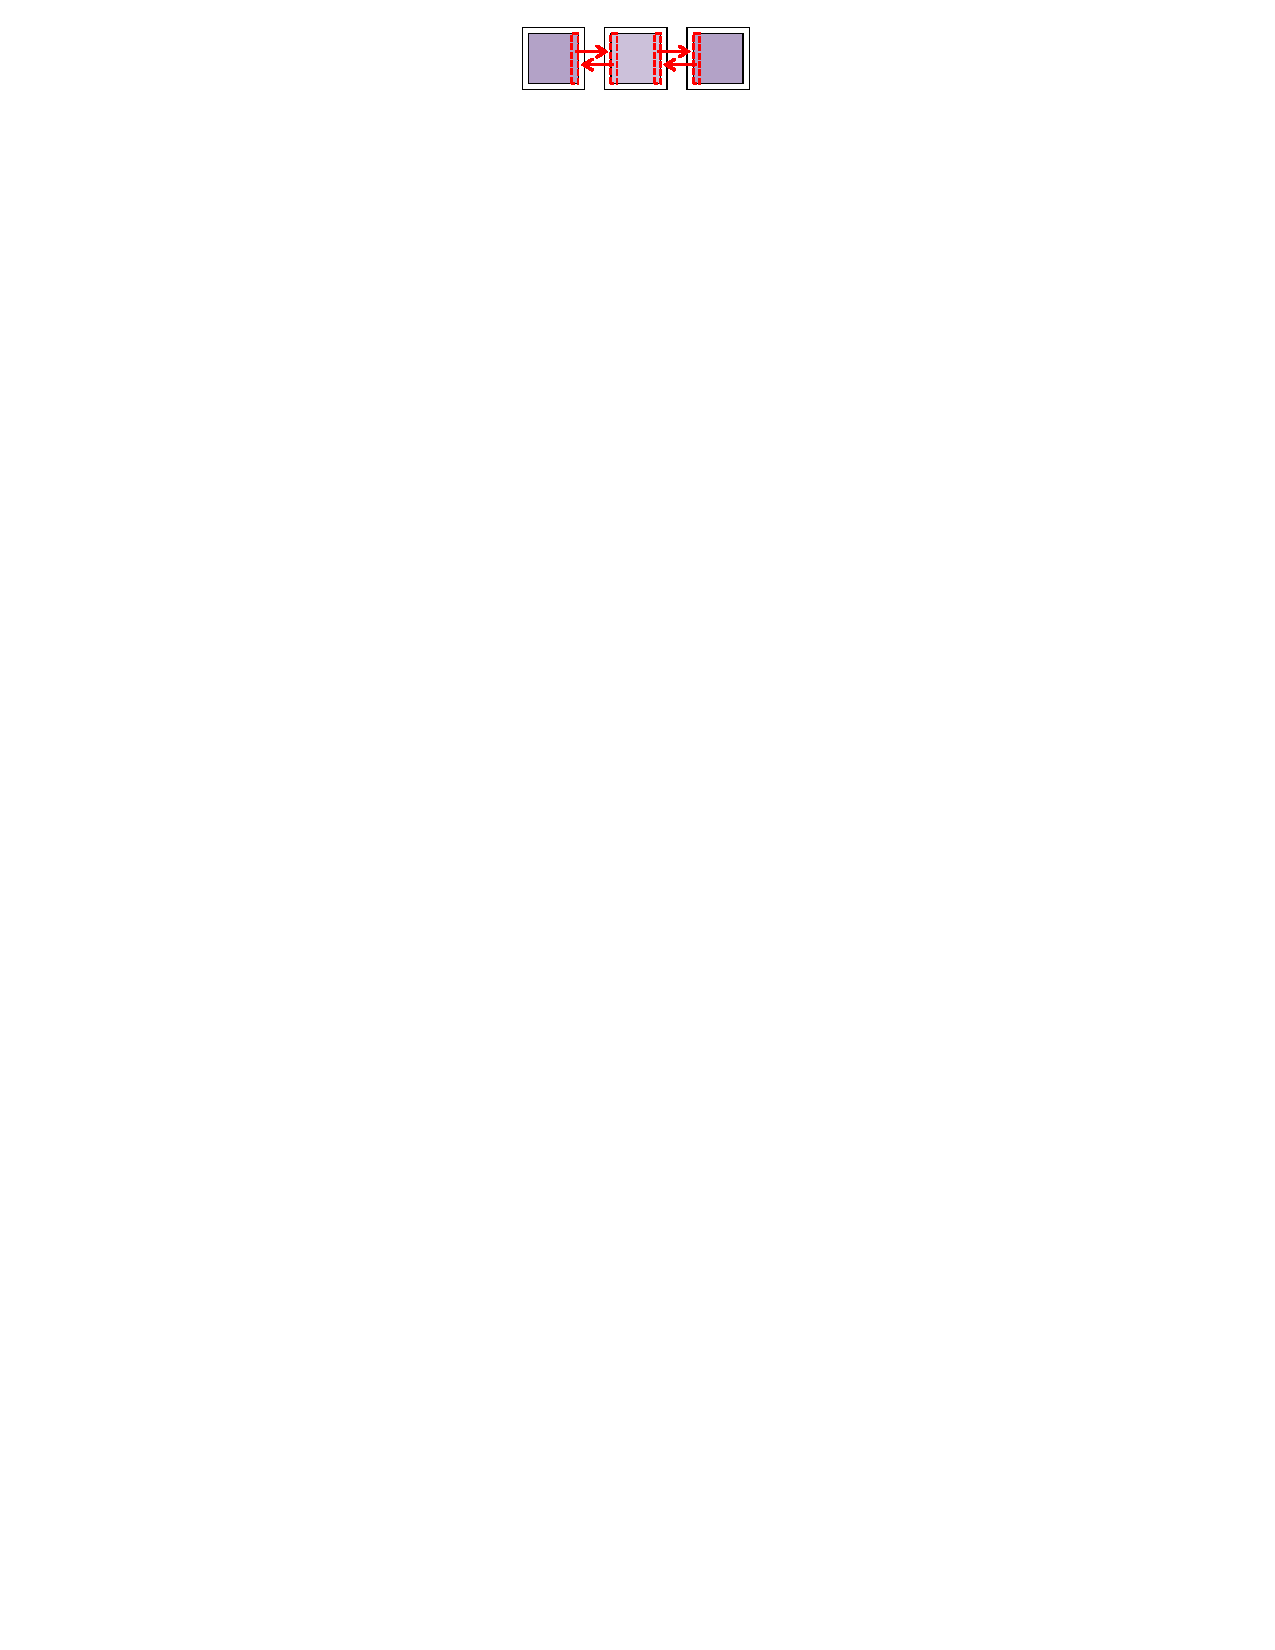
\includegraphics[trim=85mm 261mm 85mm 0mm, scale=0.8,clip]{figs/3cell-z.pdf}}  \\
  \fbox{\includegraphics[trim=82mm 230mm 84mm 0mm, scale=0.8,clip]{figs/9cell-yz.pdf}}
  \caption{3cell-y.pdf, 3cell-z.pdf, 9cell-yz.pdf}\label{fig:cell}
  \end{center}
\end{figure}


%-- 8var-pipo-latency.pdf
\begin{figure}[tbh]
  \begin{center}
  % trimはleft bottom right topの順
    \fbox{\includegraphics[trim=40mm 180mm 43mm 0mm, scale=0.8,clip]{figs/8var-pipo-bw.pdf}}
    \caption{8var-pipo-bw.pdf}\label{fig:8var-pipo-bw}
  \end{center}
\end{figure}

%-- 8var-pipo-latency.pdf
\begin{figure}[tbh]
  \begin{center}
  % trimはleft bottom right topの順
    \fbox{\includegraphics[trim=40mm 155mm 40mm 0mm, scale=0.8,clip]{figs/8var-pipo-latency.pdf}}
    \caption{8var-pipo-latency.pdf}\label{fig:8var-pipo-latency}
  \end{center}
\end{figure}

%-- HAPACS-bw.pdf
\begin{figure}[tbh]
  \begin{center}
  % trimはleft bottom right topの順
    \fbox{\includegraphics[trim=45mm 188mm 45mm 3mm, scale=0.8,clip]{figs/HAPACS-bw.pdf}}
    \caption{HAPACS-bw.pdf}\label{fig:HAPACS-bw}
  \end{center}
\end{figure}

%-- fx100-bw.pdf
\begin{figure}[tbh]
  \begin{center}
  % trimはleft bottom right topの順
    \fbox{\includegraphics[trim=41mm 190mm 49mm 3mm, scale=0.8,clip]{figs/fx100-bw.pdf}}
    \caption{fx100-bw.pdf}\label{fig:fx100-bw}
  \end{center}
\end{figure}

%-- fx100-pipo.pdf
\begin{figure}[tbh]
  \begin{center}
    % trimはleft bottom right topの順
    \fbox{\includegraphics[trim=4mm 15mm 4mm 3mm, scale=0.9,clip]{figs/fx100-pipo.pdf}}
    \caption{fx100-pipo.pdf}\label{fig:fx100-pipo}
  \end{center}
\end{figure}

%-- himeno-K-nonblock.pdf
\begin{figure}[p]
  \begin{center}
  % trimはleft bottom right topの順
    \fbox{\includegraphics[trim=37mm 34mm 37mm 4mm, scale=0.8,clip]{figs/himeno-K-nonblock.pdf}}
    \caption{himeno-K-nonblock.pdf}\label{fig:himeno-K-nonblock}
  \end{center}
\end{figure}

%himeno.pdf
%latency-16var.pdf
%layer.pdf
%-- nonblock-fig.pdf
\begin{figure}[tbh]
  \begin{center}
  % trimはleft bottom right topの順
    \fbox{\includegraphics[trim=43mm 144mm 43mm 3mm, scale=0.8,clip]{figs/nonblock-fig.pdf}}
    \caption{nonblock-fig.pdf}\label{fig:nonblock-fig}
  \end{center}
\end{figure}

%-- pingpong-code.pdf
\begin{figure}[tbh]
  \begin{center}
  % trimはleft bottom right topの順
    \fbox{\includegraphics[trim=24mm 118mm 24mm 4mm, scale=0.7,clip]{figs/pingpong-code.pdf}}
    \caption{pingpong-code.pdf}\label{fig:pingpong-code}
  \end{center}
\end{figure}

%register-CA-tmp.pdf
%register-RA-CA-tmp.pdf
%register-RA-tmp.pdf
%softstack.pdf
%translator-tmp.pdf

%\cleardoublepage

\section{Related Work}\label{sec:related}

%-- Coarray Imprementations
The Universicy of Rice has implemented coarray features with their own extension called CAF~2.0.
It is a source-to-source compiler based on the ROSE compiler. GASNet is used as its 
communication layer.
%
Houston University depeloped UH-CAF onto the Open64-base OpenUH compiler. It supports
coarray features defined in the Fortran 2008 standard. As the communication layer,
GASNet and ARMCI can be used selectively.
%
OpenCoarrays~\cite{OpenCo} is an open-source software project. It is an library 
which can be used with GNU Fortran (gfortran) V5.1 or later. It supports coarray features
specified in Fortran 2008 and a part of Fortran 2018.  As the communiation layer,
MPICH and GASNet can be used selectively.
%
In the vendors, Cray and Intel fully and Fujitsu partially support the coarray features
specified in Fortran 2008.


task間はF2018のcoarrayにある。違いは・・・

getのnonblockingは難しい。書式上、獲得したあたいがすぐに使用されることになるため、
nonblockingのrangeを大きく取れない。
putでは完了を遅延させるのにたいし、開始を先行させる技術(prefetching)が考えられる。
Crayはそのためのdirectiveをもつ。

RiceもCrayポインタを使っている。
Crayポインタはalias analysisで性能を落とす。


\section{Future Works}\label{sec:related}

Coarray C++はObject oriented programmingになれた人には自然な実装と感じるかもしれない。
我々の目指すCoarray Cはこれとは違い、HPCプログラムをCで書いている人向けに修正を最小限
にするものである。また、coarrayを抽象性の高い概念で定義するのではなく、
単にアドレスと長さで特定できるメモリの範囲と定義したい。これによって一般の
Cプログラマがキャストや引数渡しを使って同じ領域を目的によって連続配列や多次元配列
や単に先頭アドレスへのvoidポインタなどとして自由に使い回すように扱いたい。
これは美しくはないが、Cの大きなプログラムを抱えている利用者には必要である。
仕様書の定義には曖昧さが残っているので、まだ修正が必要である。
Fortranと同じような性能が出せるもので、かつ、FortranのCoarrayとの互換性を持たせたい。

Non-blocking PUT communication 
正確な実行時判定を行うためには、現在non-blocking PUT通信中のcoarrayのアドレスのrangeと相手のimage番号を
ハッシュテーブルに記憶し、GET通信を行う前にそのrangeとimage番号に重なりがないことをチェックし、
重なりがあったらそこでPUT通信を完了させる、という方法が考えられる。
しかしこれでは、重なりが無い通常のケースでも重なりのチェックのコストが大きい。
コンパイラでの解析と動的なチェックを併用する、正確さが劣ってもより高速な方法が望ましい。


%\cleardoublepage

\input{7.concl.tex}
%\cleardoublepage

\appendix

\section{MEMO}
MPIはPGASに向かない、という論文がどこかに。

\section{Fusen}
\begin{verbatim}

synmetric memory
リモートのアドレスをローカルで計算できる
これがあるから、片側通信が。。。


下位層:通信libの差異を吸収し、上位層にプリミティブを提供する。
XMP coarray実装のプリミティブi/f
put operation
get operation
- どちらも連続データのみ/nonblocking。
sync memory operation
- 発行したputをすべてremoteに書き込み、getをすべてlocalに読み込むまで待つ。

putにはnonblocking技術:runtimeで十分
getにはprefetch技術:コンパイラ技術


生産性の観点の評価
1. リンク時にstatic配列を集めるところが対MPI片側通信で重要。言語仕様/言語処理系だからできる。単にライブラリ群/ライブラリ呼出しではできない。
2. F90配列記述がMPI_Typeの定義を不要にしている。


klogin7$ which xmpf90
~/Project/OMNI-clone/bin/xmpf90
klogin7$ xmpf90 --version
Version:1.3.1, Git Hash:4a5736e
klogin7$ 


sync memoryがいつ必要か
- ユーザ記述
- getのとき、1subarray参照に対してsyncmemoryを1回にする。
- getの前に、同じremoteアドレスへのputがあればsyncmemoryで待つ


alignmentの問題か
64バイト未満でputのlatencyが高い。
src5, RUN5で改善 ・・・しなかった
メモリ割付けのalignmentの問題ではない。
残るはTofuのputの単位の問題と推測
マスク付き書き込みになる?
この点ではRDMAよりバッファリングが有利


A Source-to-Source Translation of Coarray Fortran with MPI for High Performance
https://dl.acm.org/citation.cfm?id=3155888&dl=ACM&coll=DL

Preliminary Implementation of
Coarray Fortran Translator Based on Omni XcalableMP
https://ieeexplore.ieee.org/document/7306099

\end{verbatim}


\section{STATUS-CAF}
\input{appendix/status-caf.tex}

\section{mac-air memo}
\begin{verbatim}

introduction
coarrays in XcalableMP
support F2008 coarrays
image setをtaskに対してmap
natural extension to C
basic implementation and issues
lower-level interface
evaluation
related work
Coarray C++は
task間はF2018のcoarrayにある。違いは・・・
Crayはgetをdirectiveで実装
conclusion

implementation for high performance
static coarrayの高速化
全部まとめて先にallocするコンパイラ技術
定数評価、構造体の大きめな見積り
allocatable coarrayの高速化:lowlevelに合わせて選択
RuntimeLibShare事前に巨大領域を取る
実行時allocのコストが大きいとき
RuntimeLibAllocation実行時allocのコストが小さいとき
contiguouity検出による高速化
次元を跨ぐ連続性抽出
バッファリング
有限サイズ、基礎データから、Nlocal, Nremote, Nbufの関係でアルゴリズム
CommpilerAllocationFortranがallocateしてregisterできるとき

implementation software layer
3種:one sided, collective, atomic. このうちcollectiveとatomicはMPIの機能をそのまま使う。それ以上の工夫はない。one sidedはallocate/freeとput/getと同期。lower-level通信層のバリエーションを吸収するライブラリ層を設けた。階層の図。
次元の概念とcontiguityを上位層で解決するため結果的に必要なインタフェースは少なくなった



\end{verbatim}


\section{nigun}
\subsection{introよりrelated workの方がよいか?}



PGAS言語の一つであるCoarray Fortran(CAF)は,Fortran 2008仕様の一部として採用されたことも追い風となって,近年研究開発が盛んに進められている.フリーのものでは, Houston大学のOpenUHコンパイラを開発基盤としたUH-CAF[5]と,Rice大学のROSEコンパイラを開発基盤としたcaft[6]が有名である.近年リリースされたOpenCoarrayは,GNU gfortranにリンクできるライブラリである.我々の開発するOmni XMPもまた,CAFコンパイラとして利用することができる.ベンダではCrayとIntelが古くから提供しており,近年富士通からもリリースされている.これら3社は,Fortran 2008と2015に含まれるcoarray機能の実装をFortran2003のフル実装よりも先行させたことになる.
Omni XMPは,PCクラスタコンソーシアムのXcalableMP規格部会が制定する並列言語XcalableMP(XMP)のパイロット実装である.XMPは,FortranとCをベースとし,ディレクティブ行の挿入によって並列化を記述するが,Fortran 2008で定義されるcoarray機能も仕様として含んでいる.前者は「逐次プログラムに指示を与えて並列化する」という考え方からグローバルビューと呼ばれ,並列プログラミングが容易にできることを狙う.後者は「個々のノード(イメージ)の挙動を記述する」という考え方でローカルビューと呼ばれ,MPIに匹敵する性能がMPIよりも容易に出せることを狙っている.




                                   
\begin{thebibliography}{99}
\addcontentsline{toc}{chapter}{\bibname}
 \bibitem{xmp} XcalableMP Language Specification, \url{http://xcalablemp.org/specification.html} (2017).
 \bibitem{openacc} The OpenACC Application Programming Interface, \url{http://www.openacc.org} (2015).
 \bibitem{mpi} MPI: A Message-Passing Interface Standard, \url{http://mpi-forum.org} (2015).
 \bibitem{coarray} John Reid, JKR Associates, UK. Coarrays in the next Fortran Standard.
    ISO/IEC JTC1/SC22/WG5 N1824, April 21, 2010.
 \bibitem{coarray18} ISO/IEC TS 18508:2015, Information technology -- Additional Parallel 
    Features in Fortran, Technical Specification, December 1, 2015.
 \bibitem{F08} Fortran~2008
 \bibitem{F18} Fortran~2018

 \bibitem{Rice}
 \bibitem{HU}
 \bibitem{OpenCo} http://www.opencoarrays.org/

\end{thebibliography}

\end{document}



